\begin{section}{Problem 5}
    \begin{problem}{5}
        The following picture appears in \textsc{Matlab's} repository of images, and can be retrieved by entering 
        \begin{verbatim}
    load mandrill; 
    colormap('gray'); 
    image(X);
        \end{verbatim}
        \begin{center}
            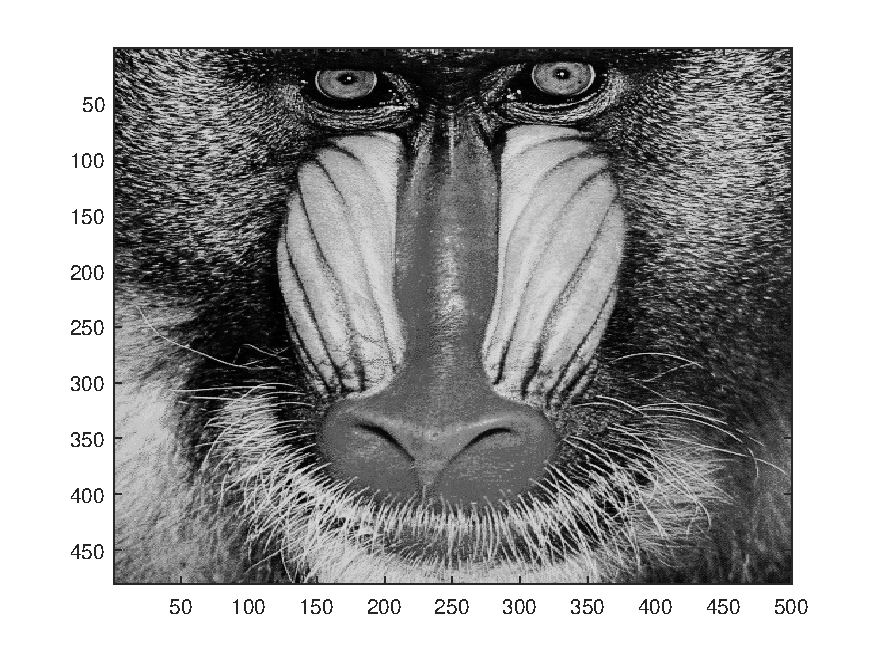
\includegraphics[scale=0.7]{mandrill2.pdf}
        \end{center}
        
        \begin{enumerate}[(a)]
            \item Print out the images generated by the truncated SVD. Start with $r=2$ and go up by powers of $2$, to $r=2^6=64$ (six plots in total). For a compact presentation of your figures, you may use the command {\tt subplot(3,2)}. (Check out {\tt help subplot}.)        
            \item Comment briefly on the quality of the images as a function of $r$. For what value of $r$ would you say that the quality of the image is acceptable, in that we can be rather confident of what we are seeing? (We are not looking for a specific ``correct answer'' here - just make your subjective observation.)
            \item For the value of $r$ you stated in part (b), how much storage is required? Compare it to the storage required for the original image.
        \end{enumerate}
    \end{problem}

    \begin{solution}{a}
        \todo{im assuming that $r$ that is the nubmer of eigenvalues}
    \end{solution}

    \newpage
    
    \begin{solution}{b}
        \todo{bullshit}
    \end{solution}

    \begin{solution}{c}
        \todo{bullshit}
    \end{solution}
\end{section}